\section{Results}
The results were achieved when training against two types of agents, random and simple agents. In figure \ref{fig:resultsrandom} the validation and training error of the agent trained against random agents is displayed.

\begin{figure}[htb]
    \centerline{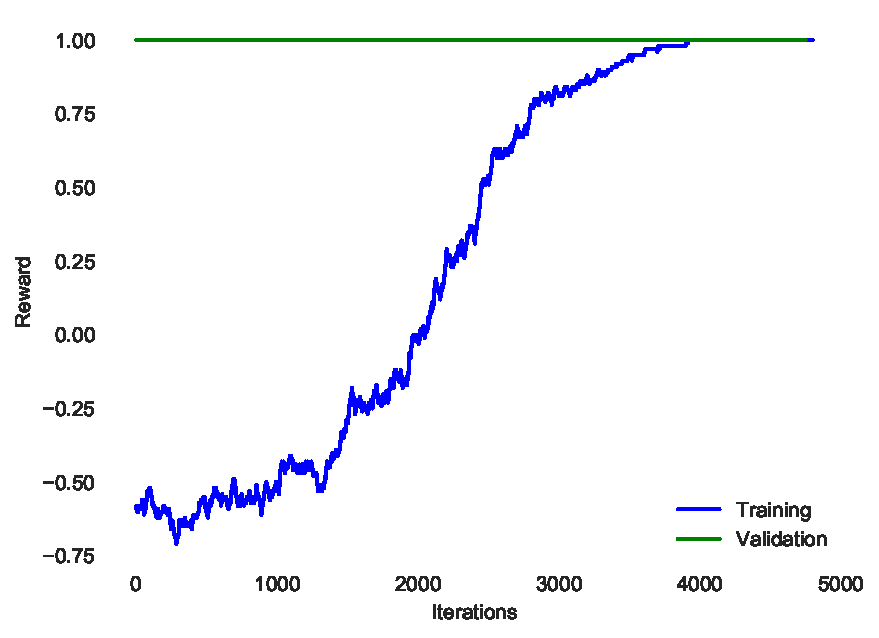
\includegraphics[width=1.0\linewidth]{docs/article/inputs/random_train_val.pdf}}
    \caption{Validation and training error against random agents.}\label{fig:resultsrandom}
\end{figure}

In figure \ref{fig:resultssimple} the validation and training error of the agent trained against simple agents is displayed. The results turned out to be independent of the reward function, furthermore the results were nearly identical regardless of using REINFORCE or Q-learning.

\begin{figure}[htb]
    \centerline{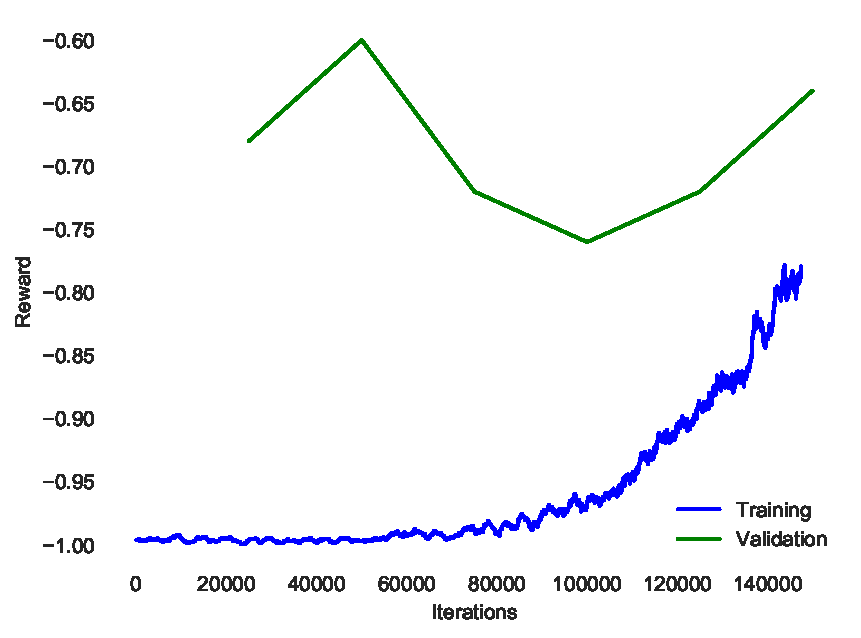
\includegraphics[width=1.0\linewidth]{docs/article/inputs/train_val.pdf}}
    \caption{Validation and training error against simple agents.}\label{fig:resultssimple}
\end{figure}

A lot of different agents were made and tested, including different hyper parameters and static board training. Each configuration was run for at least 150.000 games. However, despite these different configurations all networks ended up converging towards picking one action all the time, as is plotted in figure \ref{fig:act}. 

\begin{figure}[htb]
    \centerline{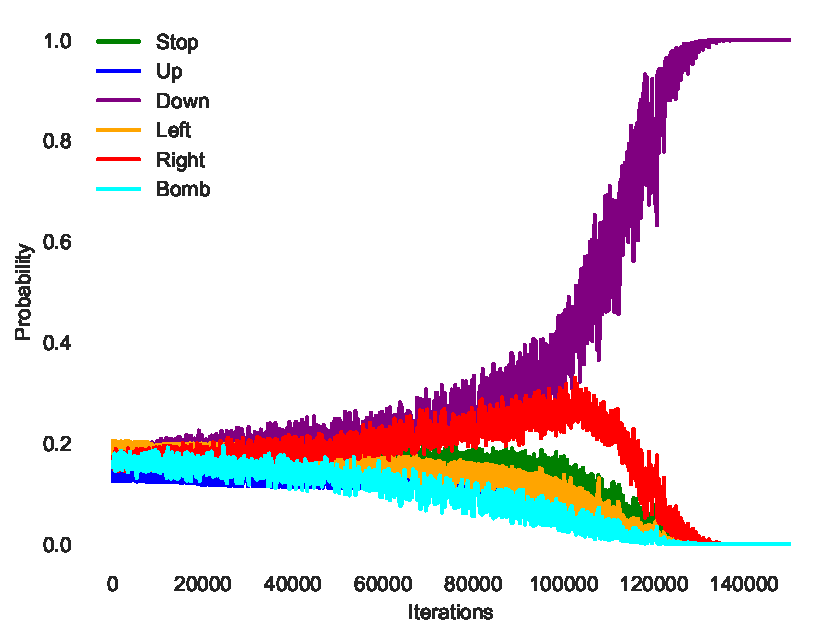
\includegraphics[width=1.0\linewidth]{docs/article/inputs/a_probs.pdf}}
    \caption{Distribution of action probabilities.}\label{fig:act}
\end{figure}







% Sometimes mentioned as experiments/results. Maybe experiments sounds better for us xD
% Show that the agent was able to learn playing against 3 random agents
% Show graphs for result for playing against 3 simple agents (-1 constantly, easy graph)

\paragraph{Performance}
% As in iterations, training time etc.
% Mention the number of iterations 

% Result for every method used should be stated